\documentclass[a4paper,11pt]{article}
\usepackage{amsmath,amsthm,amsfonts,amssymb,amscd,amstext,vmargin,graphics,graphicx,tabularx,multicol} 
\usepackage[francais]{babel}
\usepackage[utf8]{inputenc}  
\usepackage[T1]{fontenc} 
\usepackage{pstricks-add,tikz,tkz-tab,variations}
\usepackage[autolanguage,np]{numprint} 

\setmarginsrb{1.5cm}{0.5cm}{1cm}{0.5cm}{0cm}{0cm}{0cm}{0cm} %Gauche, haut, droite, haut
\newcounter{numexo}
\newcommand{\exo}[1]{\stepcounter{numexo}\noindent{\bf Exercice~\thenumexo} : \marginpar{\hfill /#1}}
\reversemarginpar


\newcounter{enumtabi}
\newcounter{enumtaba}
\newcommand{\q}{\stepcounter{enumtabi} \theenumtabi.  }
\newcommand{\qa}{\stepcounter{enumtaba} (\alph{enumtaba}) }
\newcommand{\initq}{\setcounter{enumtabi}{0}}
\newcommand{\initqa}{\setcounter{enumtaba}{0}}

\newcommand{\be}{\begin{enumerate}}
\newcommand{\ee}{\end{enumerate}}
\newcommand{\bi}{\begin{itemize}}
\newcommand{\ei}{\end{itemize}}
\newcommand{\bp}{\begin{pspicture*}}
\newcommand{\ep}{\end{pspicture*}}
\newcommand{\bt}{\begin{tabular}}
\newcommand{\et}{\end{tabular}}
\renewcommand{\tabularxcolumn}[1]{>{\centering}m{#1}} %(colonne m{} centrée, au lieu de p par défault) 
\newcommand{\tnl}{\tabularnewline}

\newcommand{\bmul}[1]{\begin{multicols}{#1}}
\newcommand{\emul}{\end{multicols}}

\newcommand{\trait}{\noindent \rule{\linewidth}{0.2mm}}
\newcommand{\hs}[1]{\hspace{#1}}
\newcommand{\vs}[1]{\vspace{#1}}

\newcommand{\N}{\mathbb{N}}
\newcommand{\Z}{\mathbb{Z}}
\newcommand{\R}{\mathbb{R}}
\newcommand{\C}{\mathbb{C}}
\newcommand{\Dcal}{\mathcal{D}}
\newcommand{\Ccal}{\mathcal{C}}
\newcommand{\mc}{\mathcal}

\newcommand{\vect}[1]{\overrightarrow{#1}}
\newcommand{\ds}{\displaystyle}
\newcommand{\eq}{\quad \Leftrightarrow \quad}
\newcommand{\vecti}{\vec{\imath}}
\newcommand{\vectj}{\vec{\jmath}}
\newcommand{\Oij}{(O;\vec{\imath}, \vec{\jmath})}
\newcommand{\OIJ}{(O;I,J)}


\newcommand{\reponse}[1][1]{%
\multido{}{#1}{\makebox[\linewidth]{\rule[0pt]{0pt}{20pt}\dotfill}
}}

\newcommand{\titre}[5] 
% #1: titre #2: haut gauche #3: bas gauche #4: haut droite #5: bas droite
{
\noindent #2 \hfill #4 \\
#3 \hfill #5

\vspace{-1.6cm}

\begin{center}\rule{6cm}{0.5mm}\end{center}
\vspace{0.2cm}
\begin{center}{\large{\textbf{#1}}}\end{center}
\begin{center}\rule{6cm}{0.5mm}\end{center}
}



\begin{document}
\pagestyle{empty}
\titre{Interrogation: Constructions de droites parallèles et perpendiculaires }{Nom :}{Prénom :}{Classe}{Date}

\vspace*{0.25cm}

\begin{flushleft}
\begin{tabular}{|m{9.5cm}|m{1.25cm}|m{1.25cm}|m{1.25cm}|m{1.25cm}|m{1.25cm}|}
\hline 
\textbf{Compétences} & \begin{center}
\textbf{N.E.}
\end{center} & \begin{center}
\textbf{M.I.}
\end{center} & \begin{center}
\textbf{M.F.}
\end{center}  & \begin{center}
\textbf{M.S.}
\end{center} & \begin{center}
\textbf{T.B.M.}
\end{center} \\ 
\hline 
Je dois connaître et savoir utiliser le vocabulaire lié à la position de deux droites (parallèle,perpendiculaire, sécante) &  &  & & &\\
\hline 
Je dois savoir tracer par un point donné la perpendiculaire à une droite donnée &  &  & & &\\
\hline 
Je dois savoir tracer par un point donné la parallèle à une droite donnée &  &  & & &\\
\hline


\end{tabular} 
\end{flushleft}

\textit{N.E = Non évalué ; M.I. = Maîtrise insuffisante ; M.F. = Maîtrise fragile ; M.S. = Maîtrise satisfaisante ; T.B.M. = Très bonne maîtrise}\\


\vspace*{0.5cm}

\exo{4} Cours \\

\q Énoncer la définition de deux droites parallèles.\\
\reponse[5]\\

\q Tracer, dans chacun des cas, la droite (d') parallèle à la droite (d) et passant par le point A.\\

\includegraphics[scale=1]{ie6.eps} \\

\medskip

\q  Tracer, dans chacun des cas, la droite (d') perpendiculaire à la droite (d) et passant par A. Coder les figures obtenues. \\


\includegraphics[scale=1]{perp.eps}\\ 

\newpage


\exo{2.5} Luc doit construire la figure ci-contre. Voici les différentes instructions mais malheureusement elles sont dans le désordre. \\
Retrouver l'ordre dans lequel il faut construire la figure.\\ 



\begin{center}
\includegraphics[scale=0.9]{programmeconstruction.eps} 
\end{center}


\bi	
\item Tracer la droite perpendiculaire à (MU) passant par I. Elle coupe (MU) en O. \fbox{\textbf{N\degre ....}}\\
\item Tracer la droite perpendiculaire à (MA) passant par U. Elle coupe (MA) en I. \fbox{\textbf{N\degre ....}}\\
\item Les droites (OH) et (IU) sont sécantes en B. \fbox{\textbf{N\degre ....}}\\
\item Tracer un triangle MAU. \fbox{\textbf{N\degre ....}}\\
\item Tracer la droite parallèle à (MA) passant par O. Elle coupe (AU) en H. \fbox{\textbf{N\degre ....}}
\ei

\exo{3}

Avec la règle et l'équerre, construire soigneusement la figure suivante.\\

\bi

\item Tracer une droite (d). Placer deux points A et L sur cette droite.

\item Placer un point $M \in (AL)$ et un point $B \notin (AL).$

\item Tracer la droite $ (d_{1})$ perpendiculaire à la droite (AL) passant par le point M.
 
\item Tracer la droite $ (d_{2})$ parallèle à la droite (AM) passant par le point B.\\

\ei

\vspace*{8cm}

\initq
\q Que peut-on dire des droites $(d_{1})$ et $(d_{2})$ ?
\reponse[2]\\

\q \textbf{BONUS } : Prouver votre dernière réponse.
\reponse[4]\\

\end{document}
